% Generado por analysis/src/tablas/figuras_tex.py — no editar a mano.
\begin{figure}[!tbp]
\centering
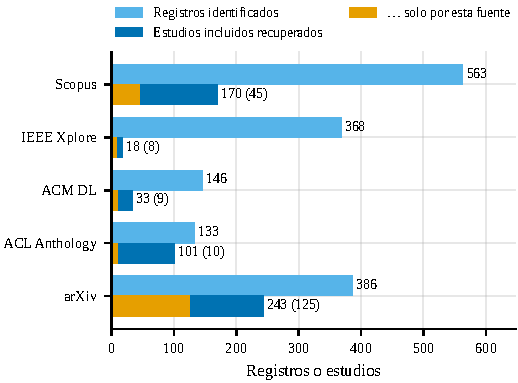
\includegraphics[width=\columnwidth,height=0.85\textheight,keepaspectratio]{busqueda_fuentes}
\caption{Registros identificados por fuente y estudios incluidos (brazo de bases) recuperados por cada fuente; entre paréntesis, los recuperados solo por esa fuente. Un estudio recuperado por varias fuentes cuenta en cada una; a cada registro conservado se le suman las fuentes de las versiones eliminadas antes del cribado.}
\label{fig:busqueda_fuentes}
\end{figure}
